\documentclass{beamer}
\setbeamertemplate{navigation symbols}{}
\usepackage[utf8]{inputenc}
\usepackage[style=verbose]{biblatex}

\title{A talk that will soon unravel\\{\small But it will try not to repeat itself}}
\author{Dan Marsden}
\date{August 2020}

\usepackage{amsmath, amsthm, amsfonts, amssymb, stmaryrd}

\usepackage{tikz}
\usepackage{tikz-cd}

\newcommand{\ie}{\textit{i.e.}~}
\newcommand{\eg}{e.g.~}
\newcommand{\Fraisse}{Fra\"{i}ss\'{e}}
\newcommand{\set}{\mathsf{set}}
\newcommand{\GS}{S}
\newcommand{\As}{\mathcal{A}}
\newcommand{\Aso}{(\As, a_0)}
\newcommand{\Bs}{\mathcal{B}}
\newcommand{\Bso}{(\Bs, b_0)}
\newcommand{\Rs}{\mathcal{R}}
\newcommand{\Tr}{\mathsf{Tr}}
\newcommand{\preord}{\preceq}
\newcommand{\preford}{\sqsubseteq}
\newcommand{\op}{\mathsf{op}}
\newcommand{\Gd}{\mathbb{G}}
\newcommand{\Gk}{\mathbb{G}_{k}}
\newcommand{\Ek}{\mathbb{E}_{k}}
\newcommand{\Pk}{\mathbb{P}_{k}}
\newcommand{\Pd}{\mathbb{T}}
\newcommand{\IFF}{\Longleftrightarrow}
\newcommand{\rarr}{\rightarrow}
\newcommand{\id}{\mathsf{id}}
\newcommand{\sg}{\sigma}
\newcommand{\va}{\vec{a}}
\newcommand{\vb}{\vec{b}}
\newcommand{\vx}{\vec{x}}
\newcommand{\vy}{\vec{y}}
\newcommand{\vz}{\vec{z}}
\newcommand{\RA}{R^{\As}}
\newcommand{\RGA}{R^{\GG \As}}
\newcommand{\RB}{R^{\Bs}}
\newcommand{\RAB}{R^{\As \times \Bs}}
\newcommand{\ve}{\varepsilon}
\newcommand{\vempty}{\varnothing}
\newcommand{\vphi}{\varphi}
\newcommand{\gsim}{\preceq^{\gd}}
\newcommand{\gsimk}{\preceq^{\gd}_{k}}
\newcommand{\gbsim}{\sim^{\gd}}
\newcommand{\gbsimk}{\sim^{\gd}_{k}}
\newcommand{\vsa}{\vspace{.1in}}
\newcommand{\RS}{\mathcal{R}(\sg)}
\newcommand{\RSI}{\mathcal{R}(\sg +I)}
\newcommand{\RSIe}{\mathcal{R}(\sg +I^{=})}
\newcommand{\pref}{\sqsubseteq}
\newcommand{\upset}{{\uparrow}}
\newcommand{\downset}{{\downarrow}}
\newcommand{\covers}{\prec}
\newcommand{\IMP}{\; \Rightarrow \;}
\newcommand{\AND}{\; \wedge \;}
\newcommand{\Nat}{\mathbb{N}}
\newcommand{\Ss}{\mathscr{S}}
\newcommand{\incarrow}{\hookrightarrow}
\newcommand{\IGA}{I^{\Gd \As}}
\newcommand{\IGAB}{I^{\Gd (\As \times \Bs)}}
\newcommand{\RGAB}{R^{\Gd (\As \times \Bs)}}
\newcommand{\CS}{\mathsf{Struct}(\sg)}
\newcommand{\clique}{\mathsf{clique}}
\newcommand{\gd}{\mathfrak{g}}
\newcommand{\Gg}{\mathbb{G}^{\gd}}
\newcommand{\Gkg}{\mathbb{G}_{k}^{\gd}}
\newcommand{\GG}{\mathbb{G}}
\newcommand{\lb}{\llparenthesis}
\newcommand{\rb}{\rrparenthesis}
\newcommand{\epsA}{\ve_{\As}}
\newcommand{\dg}{\dagger}
\newcommand{\lt}{\langle}
\newcommand{\rt}{\rangle}
\newcommand{\gp}{\gamma^{+}}
\newcommand{\Guarded}{\mathsf{Guarded}}
\newcommand{\EMG}{\CS^{\GG}}
\newcommand{\EMGk}{\CS^{\Gk}}
\newcommand{\lrarr}{\leftrightarrow}

%Dan stuff
\newcommand{\hgraph}{\mathsf{HGraph}}
\newcommand{\hver}[1]{V_{#1}}
\newcommand{\hedg}[1]{E_{#1}}
\newcommand{\hyp}[1]{(\hver{#1},\hedg{#1})}
\newcommand{\HH}{\mathbb{H}}
\newcommand{\Hk}{\HH_{k}}
\newcommand{\until}{\mathbin{\mathbf{until}}}

\newcommand{\M}{\mathbb{M}}
\newcommand{\Mk}{\M_{k}}
\newcommand{\Mp}{\mathbb{M}^{\circlearrowright}}
\newcommand{\Mpk}{\Mp_{k}}

\newcommand{\N}{\mathbb{N}}
\newcommand{\Nk}{\N_{k}}

\newcommand{\A}{\mathbb{A}}
\newcommand{\Ak}{\A_{k}}

\newcommand{\aplayn}[1]{[a_0 \rightarrow \ldots \rightarrow a_{#1}]}
\newcommand{\aplay}{\aplayn{n}}

\newtheorem{proposition}{Proposition}

\bibliography{main}

\begin{document}

\begin{frame}
\maketitle
\end{frame}

\begin{frame}[fragile]{Motivation}
    Otto and Dawar~\footcite{Otto2004},\footcite{DawarOtto2009} prove various van Benthem / Rosen theorems via upgradings:
    \begin{columns}
    \begin{column}{0.3\textwidth}
    \begin{equation*}
    \begin{tikzcd}[arrows=-]
    \As \rar["\sim_k"] \dar["\sim"] & \Bs \dar["\sim"] \\
    \hat{\As} \rar["\dot{\equiv}"] & \hat{\Bs}
    \end{tikzcd}
    \end{equation*}
    \end{column}
    \begin{column}{0.7\textwidth}
    \begin{description}
    \item[$\sim$] Bisimilarity
    \item[$\sim_k$] A finite approximation to bisimilarity
    \item[$\dot{\equiv}$] A stronger equivalence relation
    \end{description}
    \end{column}
    \end{columns}
    \begin{block}{Simple Observations}
    To show and use these lifting theorems we need to capture various notions of bisimilarity, locality and related model construction, and their interaction.
    \end{block}
\end{frame}

\begin{frame}{The Modal (Bi)simulation Game}
    We consider pointed Kripke structure~$(\As, a_0)$:
    \begin{equation*}
        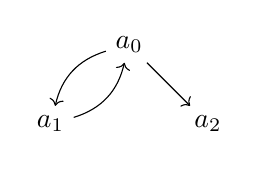
\begin{tikzpicture}
        \path node(a0) {$a_0$} +(-1,-1) node (a1) {$a_1$} +(1,-1) node(a2) {$a_2$};
        \path[->] 
        (a0) edge[bend right] (a1)
        (a1) edge[bend right] (a0)
        (a0) edge (a2);
        \end{tikzpicture}
    \end{equation*}
    \pause
    \begin{block}{Winning Strategies as Morphisms}
    We would like to build a structure~$\M \As$ such that morphisms~$\M \As \rightarrow \Bs$ correspond to winning strategies for the simulation game from~$\As$ to~$\Bs$.
    To do so, we build a structure out of valid spoiler plays, for example:
    \begin{equation*}
        [a_0 \rightarrow a_1 \rightarrow a_0 \rightarrow a_2]
    \end{equation*}
    \end{block}
\end{frame}

\begin{frame}{The Game Construction Yields an Unravelling}
    We impose a Kripke structure on the plays to force morphisms to correspond to valid Duplicator responses:
    \begin{equation*}
        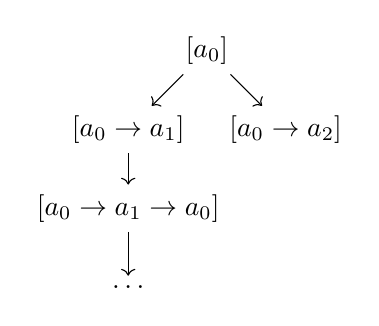
\begin{tikzpicture}
        \path 
        node (a) {$[a_0]$} +(-1,-1) 
        node (b) {$[a_0 \rightarrow a_1]$} ++(1,-1)
        node (c) {$[a_0 \rightarrow a_2]$} (b) ++(0,-1)
        node (a') {$[a_0 \rightarrow a_1 \rightarrow a_0]$} ++(0,-1)
        node (dots) {$\ldots$};
        \path[->]
        (a) edge (b)
        (a) edge (c)
        (b) edge (a')
        (a') edge (dots);
        \end{tikzpicture}
    \end{equation*}
\end{frame}

\begin{frame}{The Comonad~$\M$}
    This plan yields a comonad $\M$ with:
    \begin{description}[Kleisli co-extension:]
    \item[Object mapping:]~$(\As,a_0)$ is mapped to a structure with universe~$a_0$ rooted plays and edges:
    \begin{equation*}
        \aplay \rightarrow [a0 \rightarrow \ldots \rightarrow a_n \rightarrow a_{n + 1}]
    \end{equation*}
    \item[Counit:] The counit is the tail function:
    \begin{equation*}
        \epsilon\aplay := a_n
    \end{equation*}
    \item[Kleisli co-extension:] For~$f : \M (\As,a_0) \rightarrow (\Bs, b_0)$, we define~$f^*$ ``prefix-wise'' as follows:
    \begin{align*}
        &f^*\aplay :=\\ 
        &[f[a_0] \rightarrow \ldots \rightarrow f\aplay]
    \end{align*}
    \end{description}
\end{frame}

\begin{frame}{Polyadic Variant}
Multiple transition relations can be handled in a straightforward way by labelling:
\begin{columns}
\begin{column}{0.5\textwidth}
\begin{equation*}
    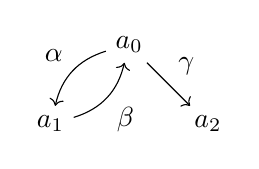
\begin{tikzpicture}
        \path node(a0) {$a_0$} +(-1,-1) node (a1) {$a_1$} +(1,-1) node(a2) {$a_2$};
        \path[->] 
        (a0) edge[bend right] node[midway, above left]{$\alpha$} (a1)
        (a1) edge[bend right] node[midway, below right]{$\beta$} (a0)
        (a0) edge node[midway, above right]{$\gamma$} (a2);
        \end{tikzpicture}
    \end{equation*}
\end{column}
\begin{column}{0.5\textwidth}
\begin{equation*}
    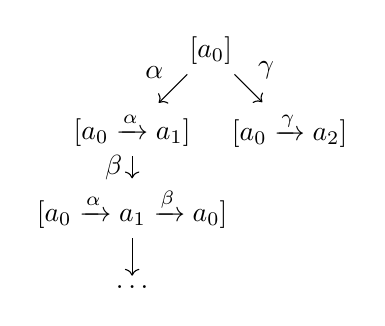
\begin{tikzpicture}
    \path 
    node (a) {$[a_0]$} +(-1,-1) 
    node (b) {$[a_0 \xrightarrow{\alpha} a_1]$} ++(1,-1)
    node (c) {$[a_0 \xrightarrow{\gamma} a_2]$} (b) ++(0,-1)
    node (a') {$[a_0 \xrightarrow{\alpha} a_1 \xrightarrow{\beta} a_0]$} ++(0,-1)
    node (dots) {$\ldots$};
    \path[->]
    (a) edge node[midway, above left]{$\alpha$} (b)
    (a) edge node[midway, above right]{$\gamma$} (c)
    (b) edge node[midway, left]{$\beta$} (a')
    (a') edge (dots);
    \end{tikzpicture}
\end{equation*}
\end{column}
\end{columns}
\pause
\begin{block}{Tree Unravelling}
$[a_0]$ is bisimilar to~$a_0$, and the construction yields a tree model. We can also grade by bounding the trees, yielding comonads~$\Mk$.
\end{block}
\end{frame}

\begin{frame}{That is not the only choice}
We can ignore the labels on paths when constructing our universe, for example:
\begin{columns}
\begin{column}{0.5\textwidth}
\begin{equation*}
    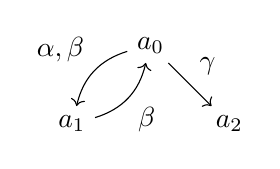
\begin{tikzpicture}
    \path node(a0) {$a_0$} +(-1,-1) node (a1) {$a_1$} +(1,-1) node(a2) {$a_2$};
    \path[->] 
    (a0) edge[bend right] node[midway, above left]{$\alpha, \beta$} (a1)
    (a1) edge[bend right] node[midway, below right]{$\beta$} (a0)
    (a0) edge node[midway, above right]{$\gamma$} (a2);
    \end{tikzpicture}
\end{equation*}
\end{column}
\begin{column}{0.5\textwidth}
\begin{equation*}
    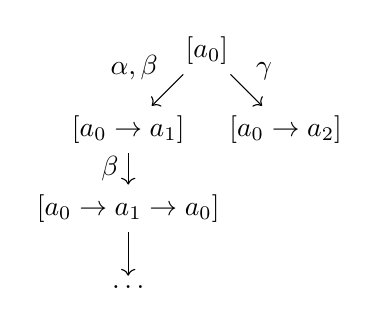
\begin{tikzpicture}
    \path 
    node (a) {$[a_0]$} +(-1,-1) 
    node (b) {$[a_0 \rightarrow a_1]$} ++(1,-1)
    node (c) {$[a_0 \rightarrow a_2]$} (b) ++(0,-1)
    node (a') {$[a_0 \rightarrow a_1 \rightarrow a_0]$} ++(0,-1)
    node (dots) {$\ldots$};
    \path[->]
    (a) edge node[midway, above left]{$\alpha, \beta$} (b)
    (a) edge node[midway, above right]{$\gamma$} (c)
    (b) edge node[midway, left]{$\beta$} (a')
    (a') edge (dots);
    \end{tikzpicture}
\end{equation*}
\end{column}
\end{columns}
We still get a tree unravelling, but with the potential for parallel edges in the Kripke structure.
\end{frame}

\begin{frame}{Another Comonad}

    \begin{proposition}
    Unlabelled directed paths yield a tree unravelling comonad.
    \end{proposition}

    \begin{block}{Comparison}
    Both constructions yield bisimilar tree unravellings:
    \begin{itemize}
        \item The original game motivated construction yields disjoint edge relations.
        \item The new construction will be trivial on tree models with parallel edges.
    \end{itemize}
    \end{block}
\end{frame}

\begin{frame}{Backwards Modalities}
    If we consider backwards modalities, we must move to two-way bisimulation. The corresponding game based construction yields for two rounds:
    \begin{columns}
    \begin{column}{0.3\textwidth}
    \begin{equation*}
    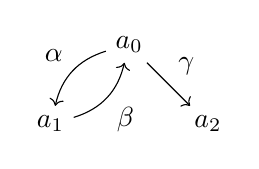
\begin{tikzpicture}
        \path node(a0) {$a_0$} +(-1,-1) node (a1) {$a_1$} +(1,-1) node(a2) {$a_2$};
        \path[->] 
        (a0) edge[bend right] node[midway, above left]{$\alpha$} (a1)
        (a1) edge[bend right] node[midway, below right]{$\beta$} (a0)
        (a0) edge node[midway, above right]{$\gamma$} (a2);
        \end{tikzpicture}
    \end{equation*}   
    \end{column}
    \begin{column}{0.7\textwidth}
    \begin{equation*}
    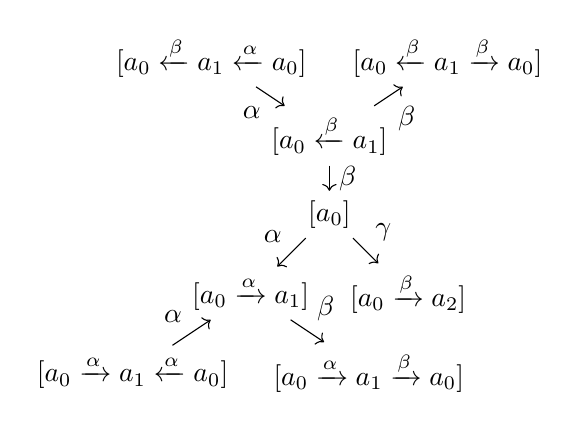
\begin{tikzpicture}
    \path 
    node (a) {$[a_0]$} +(-1,-1)
    node (b) {$[a_0 \xrightarrow {\alpha} a_1]$} +(1,-1)
    node (c) {$[a_0 \xrightarrow{\beta} a_2]$} +(0,1)
    node (d) {$[a_0 \xleftarrow{\beta} a_1]$} (b) + (-1.5,-1)
    node (e) {$[a_0 \xrightarrow{\alpha} a_1 \xleftarrow{\alpha} a_0]$} +(1.5,-1)
    node (f) {$[a_0 \xrightarrow{\alpha} a_1 \xrightarrow{\beta} a_0]$} (d) +(-1.5,1)
    node (g) {$[a_0 \xleftarrow{\beta} a_1 \xleftarrow{\alpha} a_0]$} +(1.5,1)
    node (h) {$[a_0 \xleftarrow{\beta} a_1 \xrightarrow{\beta} a_0]$};
    \path[->]
    (a) edge node[midway, above left]{$\alpha$} (b)
    (a) edge node[midway, above right]{$\gamma$} (c)
    (d) edge node[midway, right]{$\beta$} (a)
    (e) edge node[midway, above left]{$\alpha$} (b)
    (b) edge node[midway, above right]{$\beta$} (f)
    (g) edge node[midway, below left]{$\alpha$} (d)
    (d) edge node[midway, below right]{$\beta$} (h);
    \end{tikzpicture}  
    \end{equation*}
    \end{column}
    \end{columns}
\end{frame}

\begin{frame}{Two variants}
    For sequences such as~$[a_0 \xrightarrow{\alpha} a_1 \xleftarrow{\beta} a_2]$,
    we two potential modifications:
    \begin{enumerate}
        \item Removing edge orientation
        \item Removing edge labels
    \end{enumerate}
    \begin{proposition}
    Each of the four possible variants yields a comonad on pointed Kripke structures yielding two-way bisimilar tree unravellings.
    \end{proposition}
    \begin{block}{Comparison}
    We note that:
    \begin{itemize}
        \item Edge labels produce disjoint transition relations
        \item Oriented edges produce anti-symmetric (and irreflexive) edge relations
    \end{itemize}
    \end{block}
\end{frame}

\begin{frame}{A Subtlety}
Otto suggests a tree unravelling in terms of undirected paths, \emph{but} he discards ``trivial'' paths analogous to:
\begin{equation*}
    [a \rightarrow b \leftarrow a]
\end{equation*}
This prevents acyclic structures having infinite unravellings. (Is this the original motivation?).
\pause
Possibly a comonad?
\end{frame}

\begin{frame}{Unravelling a bit}
If we want to remain within finite structures, we cannot have fully bisimilar tree unravellings. Instead, we can only partially unravel:
\begin{columns}
\begin{column}{0.5\textwidth}
\begin{equation*}
        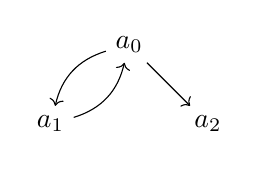
\begin{tikzpicture}
        \path node(a0) {$a_0$} +(-1,-1) node (a1) {$a_1$} +(1,-1) node(a2) {$a_2$};
        \path[->] 
        (a0) edge[bend right] (a1)
        (a1) edge[bend right] (a0)
        (a0) edge (a2);
        \end{tikzpicture}
    \end{equation*}
\end{column}
\begin{column}{0.5\textwidth}
\begin{equation*}
        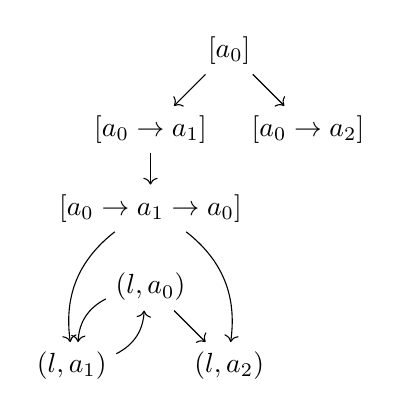
\begin{tikzpicture}
        \path 
        node (a) {$[a_0]$} +(-1,-1) 
        node (b) {$[a_0 \rightarrow a_1]$} ++(1,-1)
        node (c) {$[a_0 \rightarrow a_2]$} (b) ++(0,-1)
        node (a') {$[a_0 \rightarrow a_1 \rightarrow a_0]$} ++(0,-1)
        node (a'') {$(l, a_0)$} +(-1,-1)
        node (b'') {$(l, a_1)$} +(1,-1)
        node (c'') {$(l, a_2)$};
        \path[->]
        (a) edge (b)
        (a) edge (c)
        (b) edge (a')
        (a') edge[bend right] (b'')
        (a') edge[bend left] (c'')
        (a'') edge[bend right] (b'')
        (b'') edge[bend right] (a'')
        (a'') edge (c'');
        \end{tikzpicture}
    \end{equation*}
    Where~$l = [a_0 \rightarrow a_1 \rightarrow a_0]$
\end{column}
\end{columns}    
    
\end{frame}

\begin{frame}{Comonads again}
    \begin{proposition}
    Partial unravelling to depth~$k$ yields a comonad on (finite) pointed Kripke structures.
    \end{proposition}
    \begin{block}{Remarks}
    We can consider variations for one-way / two-way and different unravelling constructions. {\bf Details to be fully checked!}
    \end{block}
\end{frame}

\begin{frame}{Acyclicity}
\begin{block}{Bounded acyclicity}
We observe that:
\begin{itemize}
\item Full unravelling is bisimilar, completely acyclic, but out of reach for finite models.
\item Bounded unravelling is finite, but only preserves a limited depth of bisimilarity
\item The models produced by the partial unravelling are acyclic locally around the point~$a_0$
\end{itemize}
How can we achieve some acyclicity more uniformly within bisimilar finite models?
\end{block}
\end{frame}

\begin{frame}{Acyclicity Construction in Two Steps}
    Our example (no longer pointed) system:
    \begin{equation*}
        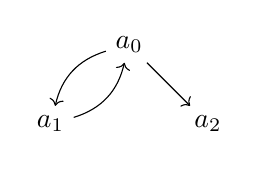
\begin{tikzpicture}
        \path node(a0) {$a_0$} +(-1,-1) node (a1) {$a_1$} +(1,-1) node(a2) {$a_2$};
        \path[->] 
        (a0) edge[bend right] (a1)
        (a1) edge[bend right] (a0)
        (a0) edge (a2);
        \end{tikzpicture}
    \end{equation*}
    Construction:
    \begin{equation*}
        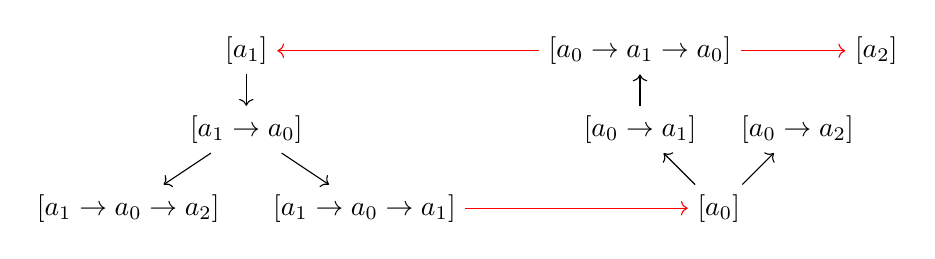
\begin{tikzpicture}
        \uncover{1-}{
        \path 
        node (a) {$[a_0]$} +(-1,1) 
        node (b) {$[a_0 \rightarrow a_1]$} ++(1,1)
        node (c) {$[a_0 \rightarrow a_2]$} (b) ++(0,1)
        node (a') {$[a_0 \rightarrow a_1 \rightarrow a_0]$} (a) ++(-6,2)
        node (b'') {$[a_1]$} ++(0,-1)
        node (a'') {$[a_1 \rightarrow a_0]$} +(1.5,-1)
        node (b''') {$[a_1 \rightarrow a_0 \rightarrow a_1]$} +(-1.5,-1)
        node (c'') {$[a_1 \rightarrow a_0 \rightarrow a_2]$} (a) ++(2,2)
        node (c''') {$[a_2]$};
        
        \path[->]
        (a) edge (b)
        (a) edge (c)
        (b) edge (a')
        (b'') edge (a'')
        (a'') edge (b''')
        (a'') edge (c'');
        }
        
        \uncover<2>{
        \path[->, red]
        (a') edge (b'')
        (a') edge (c''')
        (b''') edge (a);
        }
        \end{tikzpicture}
    \end{equation*}
\end{frame}

\begin{frame}{Yet Another Comonad}
    \begin{proposition}
    The bounded unravelling acyclicity construction yields a comonad on (finite) Kripke structures.
    \end{proposition}
    \begin{block}{Remarks}
    Lots of variants based on the previous observations. {\bf Lots of details to check!}
    \end{block}
\end{frame}

\begin{frame}{Further steps}
    \begin{itemize}
        \item There is a local neighbourhood comonad on pointed structures, relate this to the other constructions.
        \item Explain the relationship between the different variants. Here there's a potential ``disjointing'' comonad, can this be used to construct some variants in a uniform way? Is there a ``anti-symmetry'' comonad that could be used similarly?
        \item Note there seem to be some monads about as well - filtration, ultrafilter construction, ultraproducts (see for example Leinster)...
        \pause
        \item Get back to what I'm supposed to be doing - develop van Benthem - Rosen style arguments in our framework.
        \pause
        \item Get back to what I'm really supposed to be doing - understand acyclicity and its relationship to Otto's amalgamation constructions in our setting.
    \end{itemize}
\end{frame}

\end{document}
